\chapter{Reproducción de algoritmos de PCL: Visualización de nubes y extracción de keypoints}

Puesto que el código escrito en cualquier lenguaje de programación puede resultar complicado de transmitir, la forma de proceder para conseguir dicho objetivo será la siguiente; En primer lugar se explicará en alto nivel el programa en cuestión sin necesidad de leer código y haciendo uso de flujogramas u otros métodos que se consideren adecuados. Después, habiendo entendido la funcionalidad del programa, se pasará a explicar el código que lo compone con el nivel de detalle adecuado en cada momento. Para esto, también aparecerán flujogramas así como la explicación de las distintas partes del programa por parte del autor.  

\section{Visualización de nubes de puntos}
Tal y como se ha mencionado en el apartado de objetivos del presente trabajo, la visualización de nubes se considera un hito transversal pero que a la vez involucra todo el proyecto ya que es la parte más amigable al ojo humano para estudiar resultados. De este modo se aprovecha el libre uso de la documentación y los tutoriales ofrecidos por PCL para modificar el código a favor de los objetivos planteados en el TFG.
Se recuerda que la visualización de nubes no puede llevarse a cabo en la FPGA sobre la que se implementan los objetivos principales del trabajo ya que ésta no dispone de interfaz gráfica.
%http://pointclouds.org/documentation/tutorials/

Para la visualización básica de nubes de puntos se necesita en primer lugar hacer uso del módulo IO que permite leer nubes en formato PCD. Cuando la nube está cargada, utilizando el módulo visualization, se crea una nueva ventana que hace de visualizador y en la que aparecen los tres ejes coordenados XYZ y el conjunto de puntos que conforman la nube situados en el espacio respecto al origen de los mencionados ejes. Cuando el usuario lo desee, puede cerrar la ventana que el programa ha creado para terminarlo.
Este conjunto de operaciones se muestran en su explicación en alto nivel en forma de flujograma en la figura \ref{fig:visualization_diagram}

\begin{figure}
\centering
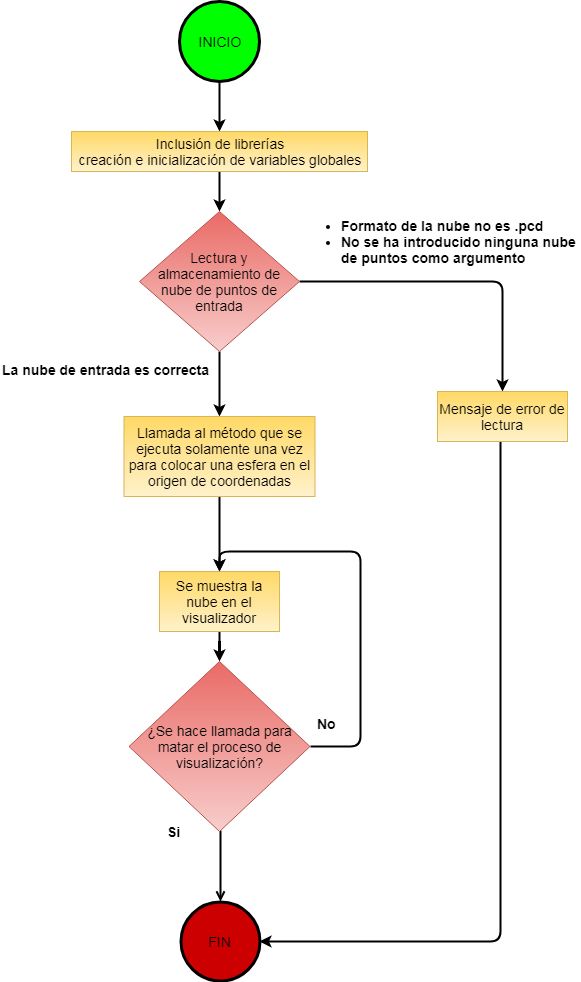
\includegraphics[scale=0.5]{visualization_diagram}
\caption{Flujograma del proceso de visualización de nubes de puntos.}\label{fig:visualization_diagram}
\end{figure}

El funcionamiento de este programa es bastante sencillo. Véase a continuación el código que hace posible la funcionalidad ya explicada.


\begin{lstlisting}[language=C++,breaklines]
#include <iostream>
#include <pcl/visualization/cloud_viewer.h>
#include <pcl/io/io.h>
#include <pcl/io/pcd_io.h>
#include <pcl/console/parse.h>
    
void 
viewerOneOff (pcl::visualization::PCLVisualizer& viewer)
{
    viewer.setBackgroundColor (1.0, 0.5, 0.5);
    pcl::PointXYZ o;
    o.x = 0;
    o.y = 0;
    o.z = 0;
    viewer.addSphere (o, 0.01, "sphere", 0); 
}
    
int 
main (int argc, char** argv)
{   

    pcl::PointCloud<pcl::PointXYZRGBA>::Ptr cloud (new pcl::PointCloud<pcl::PointXYZRGBA>);
    std::vector<int> pcd_filename_indices = pcl::console::parse_file_extension_argument (argc, argv, "pcd"); 
    std::string filename;
     
    if (!pcd_filename_indices.empty ())
    {
    	filename = argv[pcd_filename_indices[0]];
    	if (pcl::io::loadPCDFile (filename, *cloud) == -1)
    	{
      		cerr << "Was not able to open file \""<<filename<<"\".\n";
      		return -1;
    	}
    }
    else
    {
    	cout << "\nNo *.pcd file given => closing.\n\n";
    	return -1;
    }
    
    cout << "\nNumber of points in "<< filename << ": " << cloud->points.size() << "\n";
        
    pcl::visualization::CloudViewer viewer("Cloud Viewer");
    viewer.showCloud(cloud);
    
    viewer.runOnVisualizationThreadOnce (viewerOneOff);
    
    while (!viewer.wasStopped ())
    {
    }
    return 0;
}
\end{lstlisting}


En primer lugar, se cargan las librerías de iostream para las funcionalidades básicas de C++ y determinados módulos de la librería PCL; $IO$ par ala lectura de nubes, $cloud_viewer$ del módulo visualization para la visualización de nubes y $parse$ del módulo console para poder evaluar los argumentos introducidos por la consola de comandos.

\begin{lstlisting}[language=C++,breaklines]
#include <iostream>
#include <pcl/visualization/cloud_viewer.h>
#include <pcl/io/io.h>
#include <pcl/io/pcd_io.h>
#include <pcl/console/parse.h>
\end{lstlisting}


En el siguiente fragmento de código se implementa la función que se ejecutará una sola vez cuando se abre la ventana que visualiza la nube de puntos. Su funcionalidad, tal y como adelanta el flujograma ya expuesto, se basa en añadir una esfera en el origen de coordenadas para localizarlo fácilmente. Se trata del objeto $o$ de la clase $PointXYZ$ creado en la línea . Además, en la línea  se configura el color de fondo del visualizador aportando pesos a los valores máximos de color rojo, verde y azul que se pueden tener; 1.0 para el color rojo y 0.5 para los colores verde y azul. Finalmente, con el método $addSphere$ se añade al visualizador a esfera creada.
\begin{lstlisting}[language=C++,breaklines]
void 
viewerOneOff (pcl::visualization::PCLVisualizer& viewer)
{
    viewer.setBackgroundColor (1.0, 0.5, 0.5);
    pcl::PointXYZ o;
    o.x = 0;
    o.y = 0;
    o.z = 0;
    viewer.addSphere (o, 0.01, "sphere", 0); 
}
\end{lstlisting}


A continuación, dentro del método principal $main$, se crea un objeto de nube de puntos llamado $cloud$ que contiene información de coordenadas XYZ y color RGBA, refiriéndose RGB a Red, Green y Blue respectivamente, es decir, rojo, verde y azul. la letra $A$ se refiere a la intensidad de color. 
También se crea el objeto $pcd_filename_indices$ que guarda el índice del argumento pasado por consola de comandos que contiene la nube de puntos en formato PCD. En $filename$ se guarda el nombre de la nube de puntos.
Si $pcd_filename_indices$ está vacío quiere decir que el usuario no ha introducido ninguna nube de puntos en formato PCD por lo que el programa termina en este punto con el mensaje de error correspondiente. En caso contrario, se procede a leer y almacenar la nube de puntos de entrada y si el método de lectura falla, el programa termina con el mensaje de error correspondiente.
Si todo va bien y se consigue leer la nube y almacenarla en el objeto $cloud$, a modo informativo, se muestra por pantalla el número de puntos que contiene la nube accediendo al atributo SIZE de la misma (referencia a formato PCD)


\begin{lstlisting}[language=C++,breaklines]
int 
main (int argc, char** argv)
{   

    pcl::PointCloud<pcl::PointXYZRGBA>::Ptr cloud (new pcl::PointCloud<pcl::PointXYZRGBA>);
    std::vector<int> pcd_filename_indices = pcl::console::parse_file_extension_argument (argc, argv, "pcd"); 
    std::string filename;
     
    if (!pcd_filename_indices.empty ())
    {
    	filename = argv[pcd_filename_indices[0]];
    	if (pcl::io::loadPCDFile (filename, *cloud) == -1)
    	{
      		cerr << "Was not able to open file \""<<filename<<"\".\n";
      		return -1;
    	}
    }
    else
    {
    	cout << "\nNo *.pcd file given => closing.\n\n";
    	return -1;
    }
    
    cout << "\nNumber of points in "<< filename << ": " << cloud->points.size() << "\n";
\end{lstlisting}

Por último, se crea un objeto de visualización llamado $viewer$ y el cual se utiliza para mostrar la nube con la llamada a $showcloud$ y asignar el método $runOnVisualizationThreadOnce$ explicado previamente para ejecutarse al comienzo de la visualización de la nube. 
Siempre y cuando el proceso de visualización no haya sido detenido, la nube seguirá mostrándose por la ventana creada para este propósito. Esto se consigue con el bucle $while$

\begin{lstlisting}[language=C++,breaklines]
	pcl::visualization::CloudViewer viewer("Cloud Viewer");
    viewer.showCloud(cloud);
    viewer.runOnVisualizationThreadOnce (viewerOneOff);
    
    while (!viewer.wasStopped ())
    {
    }
    return 0;
}
\end{lstlisting}

el otro vsiualizadooooooooooooooooooor

el programa principaaaaaaaaaaaaaaaaaaaaaaal

\begin{lstlisting}[language=C++,breaklines]

// STL
#include <iostream>

// PCL
#include <pcl/io/pcd_io.h>
#include <pcl/io/impl/pcd_io.hpp>

#include <pcl/point_types.h>

#include <pcl/common/io.h>

#include <pcl/keypoints/sift_keypoint.h>
#include <pcl/keypoints/narf_keypoint.h>
#include <pcl/features/normal_3d.h>
#include <pcl/features/impl/normal_3d.hpp>

#include <pcl/impl/pcl_base.hpp>

#include <pcl/search/pcl_search.h>
#include <pcl/search/impl/search.hpp>
#include <pcl/search/impl/organized.hpp>
#include <pcl/search/impl/kdtree.hpp>

#include <pcl/filters/impl/voxel_grid.hpp>

#include <pcl/kdtree/impl/kdtree_flann.hpp>

#include <ctime>

#include <boost/thread/thread.hpp>

#include <pcl/features/normal_3d_omp.h>

#include <pcl/console/parse.h>

#include <fstream>

int normal_estimation_object = 0;
float radius_search = 0.02f;
float normal_estimation_time = 0.0f;
float sift_estimation_time = 0.0f;

float min_scale = 0.01f;
int n_octaves = 3;
int n_scales_per_octave = 4;
float min_contrast = 0.001f;
int sift_points=0; 

clock_t begin,end;
double elapsed_sec;

void 
printUsage (const char* progName)
{
  std::cout << "\n\nUsage: "<<progName<<" [options] <scene.pcd>\n\n"
            << "Options:\n"
            << "-------------------------------------------\n"
            << "-o <integer>	0 for regular normal estimation (default), 1 for enhanced normal estimation\n"
            << "-r <float>	Radius search for normal estimation (default "<< radius_search<<")\n"
            << "-ms <float>	Minimum scale (default " << min_scale << ")\n"
            << "-no <int>	Number of octaves (default " << n_octaves << ")\n"
            << "-ns <int>	Number of scales per octave (default " << n_scales_per_octave << ")\n"
	    << "-mc <float>	Minimum contrast (default " << min_contrast << ")\n"
	    << "-h		Show help\n"
            << "\n\n";
}

int main(int argc, char** argv)
{

  if(argc == 1 || (pcl::console::find_argument (argc,argv,"-h") >= 0) )
  {
	printUsage (argv[0]);
	return 0;
  }	

  std::cout << std::endl << "---Normal estimation parameters---" << std::endl;

  pcl::NormalEstimation<pcl::PointXYZ, pcl::PointNormal> ne;
  pcl::console::parse (argc, argv, "-o", normal_estimation_object);
  if(normal_estimation_object >0)
  {
	std::cout << "Using enhanced normal estimation object" << std::endl;
	pcl::NormalEstimationOMP<pcl::PointXYZ, pcl::PointNormal> ne;
  }
  else
  {
	std::cout << "Using regular normal estimation object" << std::endl;
  }
  
  pcl::console::parse (argc,argv, "-r", radius_search);
  std::cout << "Setting radius search for normal estimation to: " << radius_search << std::endl;

  
  std::cout << std::endl << "---Sift points parameters---" << std::endl;
  
  
  pcl::console::parse (argc,argv, "-ms", min_scale);
  std::cout << "Setting minimum scale to: " << min_scale << std::endl;

  pcl::console::parse (argc,argv, "-no", n_octaves);
  std::cout << "Setting number of octaves to: " << n_octaves << std::endl;

  pcl::console::parse (argc,argv, "-ns", n_scales_per_octave);
  std::cout << "Setting number of scales per octave to: " << n_scales_per_octave << std::endl;

  pcl::console::parse (argc,argv, "-mc", min_contrast);
  std::cout << "Setting minimum contrast to: " << min_contrast << std::endl;

  std::cout << std::endl << std::endl;

  begin = clock();

  pcl::PointCloud<pcl::PointXYZ>::Ptr cloud_xyz (new pcl::PointCloud<pcl::PointXYZ>);
  std::vector<int> pcd_filename_indices = pcl::console::parse_file_extension_argument (argc, argv, "pcd"); 
  std::string filename;
     
  std::cout << "Reading file..." << std::endl;

  if (!pcd_filename_indices.empty ())
  {
  	filename = argv[pcd_filename_indices[0]];
  	if (pcl::io::loadPCDFile (filename, *cloud_xyz) == -1) 
    	{
        	std::cout << "Was not able to open file \""<<filename<<"\".\n";
       		return -1;
    	}
  }
  else
  {
  	std::cout << "\nNo *.pcd file given => closing.\n\n";
  	return -1;
  }
  
  end = clock();
  elapsed_sec = double(end-begin)/CLOCKS_PER_SEC;
  std::cout << "Number of points in "<< filename << ": "<< cloud_xyz->points.size () <<std::endl; 
  std::cout << "Time needed for " << filename << " to load: " << elapsed_sec << " seconds"<< std::endl << std::endl; 
 
  
  pcl::PointCloud<pcl::PointNormal>::Ptr cloud_normals (new 		pcl::PointCloud<pcl::PointNormal>);
  pcl::search::KdTree<pcl::PointXYZ>::Ptr tree_n(new pcl::search::KdTree<pcl::PointXYZ>());

  ne.setInputCloud(cloud_xyz);
  ne.setSearchMethod(tree_n);
  ne.setRadiusSearch(radius_search);
 
  std::cout << "Estimating normals in " << filename << " surface..." <<std::endl;

  begin = clock();
  ne.compute(*cloud_normals);
  end = clock();

  normal_estimation_time = double(end-begin)/CLOCKS_PER_SEC;
  std::cout << "Time needed for normal estimation (compute) in " << filename << ": " << normal_estimation_time << " seconds" << std::endl << std::endl;

//----Copy the xyz info from cloud_xyz and add it to cloud_normals as the xyz field in PointNormals estimation is zero---
  
  std::cout << "Copying xyz information from" << filename << " to cloud with normals information..." << std::endl;

  begin = clock();

  for(size_t i = 0; i<cloud_normals->points.size(); ++i)
  {
  	cloud_normals->points[i].x = cloud_xyz->points[i].x;
  	cloud_normals->points[i].y = cloud_xyz->points[i].y;
  	cloud_normals->points[i].z = cloud_xyz->points[i].z;
  }

  end = clock();
  elapsed_sec = double(end-begin)/CLOCKS_PER_SEC;
  std::cout << "Time needed for copying the pointcloud: " << elapsed_sec <<" seconds" << std::endl << std::endl;
  if(cloud_normals->points.size()!=0){
  	pcl::io::savePCDFileASCII ("cloud_normals.pcd", *cloud_normals);
  }

  pcl::SIFTKeypoint<pcl::PointNormal, pcl::PointWithScale> sift;
  pcl::PointCloud<pcl::PointWithScale>::Ptr result(new pcl::PointCloud<pcl::PointWithScale>);
  pcl::search::KdTree<pcl::PointNormal>::Ptr tree(new pcl::search::KdTree<pcl::PointNormal> ());
  sift.setSearchMethod(tree);
  sift.setScales(min_scale, n_octaves, n_scales_per_octave);
  sift.setMinimumContrast(min_contrast);
  sift.setInputCloud(cloud_normals);
 
  std::cout << "Estimating sift points in " << filename << "..." << std::endl;

  begin = clock();
  sift.compute(*result);
  end = clock();
  sift_estimation_time = double(end-begin)/CLOCKS_PER_SEC;
  std::cout << "Time needed for sift point extraction: " << sift_estimation_time << " seconds" << std::endl << std::endl;


  if(result->points.size()>0){
  
  	std::cout << "Number of SIFT points in " << filename << ": " << result->points.size () << std::endl;

	sift_points = result->points.size();

	pcl::PointCloud<pcl::PointXYZRGBA>::Ptr keypoints(new pcl::PointCloud<pcl::PointXYZRGBA>);
  
	keypoints->width = result->width;
	keypoints->height = result->height;
	keypoints->points.resize(keypoints->width * keypoints->height);

   	for (size_t i = 0; i < result->points.size (); ++i)
  	{
    		keypoints->points[i].x = result->points[i].x;
    		keypoints->points[i].y = result->points[i].y;
    		keypoints->points[i].z = result->points[i].z;

  		keypoints->points[i].r=50;
  		keypoints->points[i].g=255;
  		keypoints->points[i].b=50;
  		keypoints->points[i].a=255;
  	}
  	pcl::io::savePCDFileASCII ("sift_keypoints.pcd", *keypoints);
  }
  else {
  	std::cout << "No sift points found" << std::endl;
	sift_points = 0;
  }
 
  std::fstream fs;
  fs.open("tests.txt", std::fstream::app);
  
  fs << "filename: " << filename << std::endl;
  
  fs << std::endl <<  "Normal estimation radius search: " << radius_search << std::endl; 
  fs << "Minimum scale: " << min_scale << std::endl;
  fs << "Number of octaves: " << n_octaves << std::endl;
  fs << "Number of scales per octave: " << n_scales_per_octave << std::endl;
  fs << "Minimum contrast: " << min_contrast << std::endl;

  fs << std::endl << "Normal estimation time (s): " << normal_estimation_time << std::endl;
  fs << "SIFT points estimation time (s): " << sift_estimation_time << std::endl;
  fs << "Number of SIFT points found: " << sift_points << std::endl;

  fs << "---------------------\n----------------------\n";
  fs.close();
  return 0;
}
\end{lstlisting}
